% vim:encoding=utf8 ft=tex sts=2 sw=2 et:

\documentclass{classrep}
\usepackage[utf8]{inputenc}
\usepackage{fixltx2e}
\usepackage{url}
\usepackage{graphicx}
\usepackage{siunitx}

\studycycle{Informatyka, studia niestacjonarne, inż I st.}
\coursesemester{VI}

\coursename{Sztuczna inteligencja i systemy ekspertowe}
\courseyear{2013/2014}

\courseteacher{dr inż. Krzysztof Lichy}
\coursegroup{sobota, 15:30}

\author{
  \studentinfo{Łukasz Ochmański}{183566} \and
  \studentinfo{Przemysław Szwajkowski}{173524}
}

\title{Zadanie 1 - przeszukiwanie przestrzeni stanów}
\svnurl{https://sise-lukasz-ochmanski.googlecode.com/svn/trunk/}

\begin{document}
\maketitle


\section{Wprowadzenie}
Celem niniejszego zadania jest napisanie dwóch programów. Pierwszy z nich ma za zadanie odnaleźć rozwiązanie łamigłówki zwanej ``Piętnastką'', a drugi ma na celu wizualizację rozwiązywania łamigłówki.

\section{Uruchamianie programu}
Program można uruchomić z lini poleceń w systemie z zainstalowaną wirtualną maszyną Java'y wersji 7 lub nowszej. Program przyjmuje jeden parametr:

\begin{itemize}
  \item \begin{verbatim}alogorytm\end{verbatim} a do wyboru: \emph{dfs, bfs, dijkstra, a1, a2, a3}
\end{itemize}

Przed uruchomieniem należy spakować projekt wraz z bibliotekami do formatu *.jar.
Metoda main() znajduje się w pliku Solver.java
\\*

Następnie uruchomić polecenie:

\begin{verbatim}
java -jar Zadanie1.jar bfs;
\end{verbatim}
	
\section{Analiza danych}
  \subsection{DFS}
  \label{subsec:DFS}
    Algorytm przeszukiwania grafu ``w głąb'' (\textit{ang. Depth-First Search}) jest algorytmem rekurencyjnym i polega na tym, że plansza przeszukiwana jest od korzenia wzdłuż jednej gałęzi, w zadanym z góry kierunku. Kiedy algorytm dojdzie do końca gałęzi, wraca do rodzica i przechodzi do kolejnego dziecka, które także jest zdefiniowane przez kolejność.


\begin{table}
\centering
\scalebox{0.7}{
\begin{tabular}{|c||c|c|c|c|}
\hline
poziom & liczba operacji & odwiedzone węzły & czas wykonania & przeciętne rozwiązanie \\
\hline
1 &	28 & 29 &	0.005ms & 28\\
\hline
2 &	62660 &	61952 &	0.758ms & 468\\
\hline
3 & 125773 & 124339 &	1.415ms & 14494\\
\hline
4 & 183119 & 181038 &	1.820ms & 5388\\
\hline
5 & 197815 & 195536 &	2.128ms & 5610\\
\hline
6 & 235743 & 233053 &	2.503ms & 5640\\
\hline
7 & 242122 & 239335 &	2.391ms & 3930\\
\hline
8 & 238376 & 235654 &	2.664ms & 2906\\
\hline
9 & 244965 & 242148 &	2.612ms & 2935\\
\hline
10 & 232649 & 229995 & 2.890ms & 1108\\
\hline

\end{tabular} }
\caption{Depth-First Search}
\end{table}

\begin{figure}[ht]
\centering
			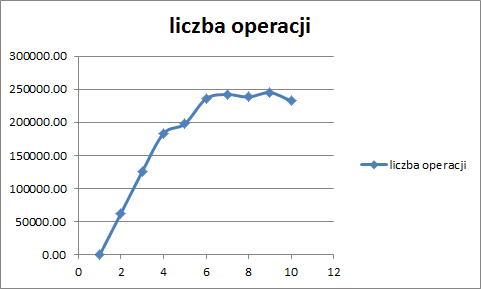
\includegraphics[scale=0.65]{pictures/dfs_operacje.png}
	\caption{Depth-First Search}
	\label{fig:Depth-First Search}
\end{figure}

\begin{figure}[ht]
\centering
			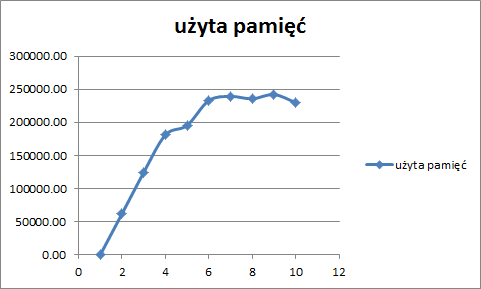
\includegraphics[scale=0.65]{pictures/dfs_space.png}
	\caption{Depth-First Search}
	\label{fig:Depth-First Search}
\end{figure}

  
    \cleardoublepage
  \subsection{BFS}
  BFS (\textit{ang. Breadth-first search}) czyli algorytm przeszukiwania grafu ``wszerz''. Algorytm ten przeszukuje cały graf wszerz aż do znalezienia węzła docelowego. W przypadku rozwiązywania łamigłówki, jego działanie polega na tym, że pobiera stan początkowy i sprawdza czy spełnia on warunek stopu. Jeżeli nie, to przechodzi do wyznaczenia wszystkich możliwych stanów potomnych zgodnie z podaną kolejnością. BFS nie wykorzystuje żadnej heurystyki.
	
		\begin{table}
\centering
\scalebox{0.7}{
\begin{tabular}{|c||c|c|c|c|}
\hline
poziom & liczba operacji & odwiedzone węzły & czas wykonania & przeciętne rozwiązanie \\
 \hline 1&	2&		3&		0.001ms	& 1\\
 \hline 2&	7&		8&		0.001ms	& 2\\
 \hline 3&	18&		19&		0.001ms & 3\\
 \hline 4&	40&		41&		0.002ms & 4\\
 \hline 5&	86&		87&		0.002ms & 5\\
 \hline 6&	191&	192&	0.002ms & 6\\
 \hline 7&	417&	418&	0.005ms & 7\\
 \hline 8&	880&	881&	0.009ms & 8\\
 \hline 9&	1894&	1895&	0.020ms & 9\\
 \hline 10&	3709&	3710&	0.041ms & 10\\
\hline

\end{tabular}}
\caption{Breadth-first search}
\end{table}

\begin{figure}[ht]
\centering
			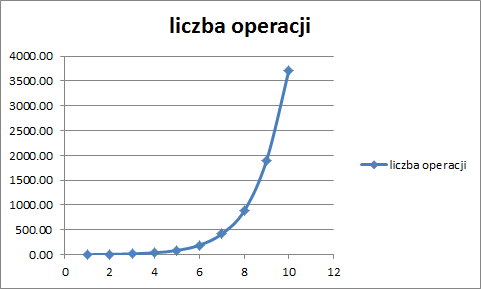
\includegraphics[scale=0.65]{pictures/bfs_operacje.png}
	\caption{Breadth-first search}
	\label{fig:Breadth-first search}
\end{figure}

\begin{figure}[ht]
\centering
			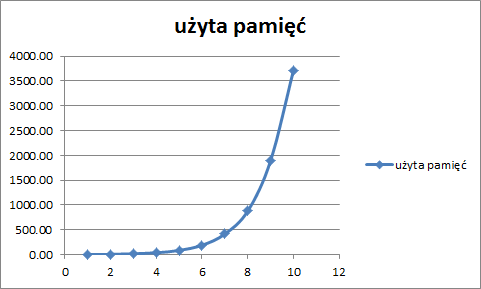
\includegraphics[scale=0.65]{pictures/bfs_space.png}
	\caption{Breadth-first search}
	\label{fig:Breadth-first search}
\end{figure}

  \cleardoublepage	
  \subsection{A* Odległość taksówkowa}
  Algorytm ten wykorzystuję heurystykę. Jego działanie polega na tym, że wybierana jest ścieżka pomiędzy wierzchołkiem początkowym, a końcowym. Wybór kolejnego elementu ścieżki uzależniony jest od wartości funkcji $f(x) = g(x) + h(x)$. Odległość taksówkowa to odległość od pustego klocka do jego docelowej pozycji. Odległość taksówkowa jest równa sumie współrzędnych w układzie kartezjańskim.
  
		\begin{table}
\centering
\scalebox{0.7}{
\begin{tabular}{|c||c|c|c|c|}
\hline
poziom & liczba operacji & odwiedzone węzły & czas wykonania & przeciętne rozwiązanie \\
\hline
\hline 1&	3&	4&	221\si{\micro\second}&	1\\
\hline 2&	7&	7&	380\si{\micro\second}&	2\\
\hline 3&	10&	9&	233\si{\micro\second}&	3\\
\hline 4&	14&	12&	224\si{\micro\second}&	4\\
\hline 5&	18&	14&	210\si{\micro\second}&	5\\
\hline 6&	23&	18&	230\si{\micro\second}&	6\\
\hline 7&	30&	23&	309\si{\micro\second}&	7\\
\hline 8&	43&	31&	348\si{\micro\second}&	8\\
\hline 9&	55&	39&	431\si{\micro\second}&	9\\
\hline 10&	79&	56&	622\si{\micro\second}&	10\\
\hline

\end{tabular}}
\caption{A* Odleglosc taksowkowa}
\end{table}

\begin{figure}[ht]
\centering
			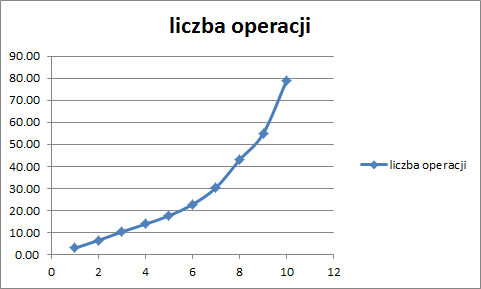
\includegraphics[scale=0.65]{pictures/A1_operacje.png}
	\caption{A* Odleglosc taksowkowa}
	\label{fig:A* Odleglosc taksowkowa}
\end{figure}

\begin{figure}[ht]
\centering
			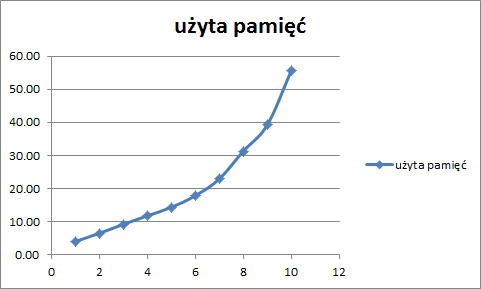
\includegraphics[scale=0.65]{pictures/A1_space.png}
	\caption{A* Odleglosc taksowkowa}
	\label{fig:A* Odleglosc taksowkowa}
\end{figure}


\cleardoublepage
  \subsection{A* Odległość Hamminga}
  Algorytm ten wykorzystuję heurystykę. Liczba klocków nie znajdująca się na swojej właściwej pozycji.
  
\begin{table}
\centering
\scalebox{0.7}{
\begin{tabular}{|c||c|c|c|c|}
\hline
poziom & liczba operacji & odwiedzone węzły & czas wykonania & przeciętne rozwiązanie \\
\hline
\hline 1&	3&	4&	1839\si{\micro\second}&	1\\
\hline 2&	9&	8&	763\si{\micro\second}&	2\\
\hline 3&	17&	14&	474\si{\micro\second}&	3\\
\hline 4&	33&	24&	558\si{\micro\second}&	4\\
\hline 5&	73&	50&	1570\si{\micro\second}&	5\\
\hline 6&	170&	114&	1540\si{\micro\second}&	6\\
\hline 7&	341&	226&	3376\si{\micro\second}&	7\\
\hline 8&	680&	446&	8783\si{\micro\second}&	8\\
\hline 9&	1425&	930&	33083\si{\micro\second}&	9\\
\hline 10&	3213&	2085&	214685\si{\micro\second}&	10.05\\
\hline

\end{tabular}}
\caption{A* Odleglosc Hamminga}
\end{table}
\begin{figure}[ht]
\centering
			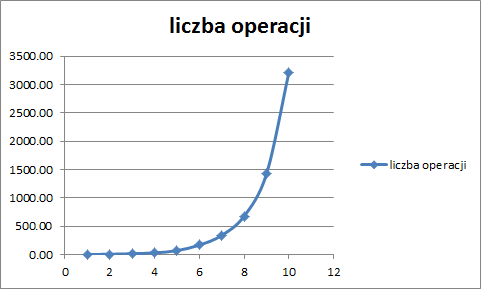
\includegraphics[scale=0.65]{pictures/A2_operacje.png}
	\caption{A* Odleglosc Hamminga}
	\label{fig:A* Odleglosc Hamminga}
\end{figure}

\begin{figure}[ht]
\centering
			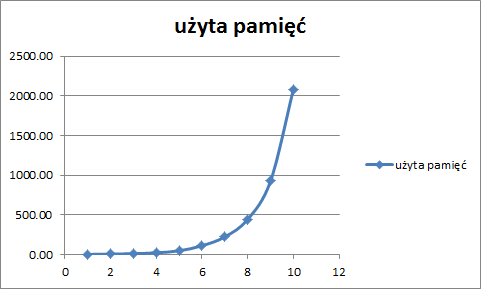
\includegraphics[scale=0.65]{pictures/A2_space.png}
	\caption{A Odleglosc Hamminga}
	\label{fig:A Odleglosc Hamminga}
\end{figure}

\cleardoublepage
  \subsection{A* Suma odległości taksówkowych}
  Algorytm ten wykorzystuję heurystykę. Odległość taksówkowa wszystkich klocków do swojej docelowej pozycji. Odległość taksówkowa jest równa sumie współrzędnych w układzie kartezjańskim.
  
\begin{table}
\centering
\scalebox{0.7}{
\begin{tabular}{|c||c|c|c|c|}
\hline
poziom & liczba operacji & odwiedzone węzły & czas wykonania & przeciętne rozwiązanie \\
\hline1&	3&	4&	260\si{\micro\second}&	1\\
\hline2&	7&	7&	460\si{\micro\second}&	2\\
\hline3&	10&	9&	454\si{\micro\second}&	3\\
\hline4&	15&	12&	271\si{\micro\second}&	4\\
\hline5&	19&	15&	215\si{\micro\second}&	5\\
\hline6&	26&	20&	265\si{\micro\second}&	6\\
\hline7&	33&	25&	330\si{\micro\second}&	7\\
\hline8&	45&	32&	381\si{\micro\second}&	8\\
\hline9&	56&	40&	528\si{\micro\second}&	9\\
\hline10&	75&	52&	681\si{\micro\second}&	10\\
\hline

\end{tabular}}
\caption{A* Suma odleglosci taksowkowych}
\end{table}

\begin{figure}[ht]
\centering
			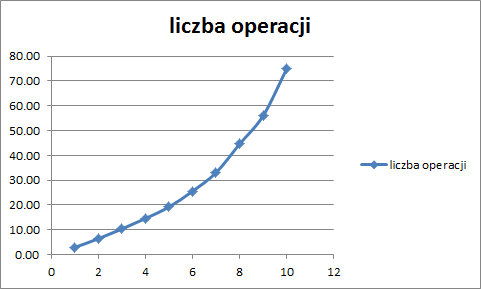
\includegraphics[scale=0.65]{pictures/A3_operacje.png}
	\caption{A* Suma odleglosci taksowkowych}
	\label{fig:A* Suma odleglosci taksowkowych}
\end{figure}

\begin{figure}[ht]
\centering
			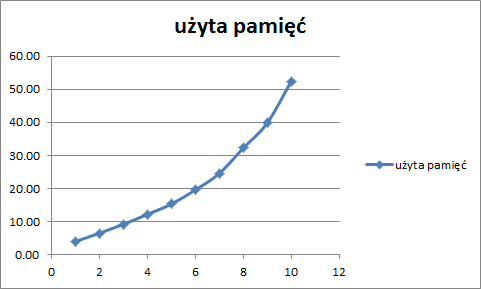
\includegraphics[scale=0.65]{pictures/A3_space.png}
	\caption{A* Suma odleglosci taksowkowych}
	\label{fig:A* Suma odleglosci taksowkowych}
\end{figure}

\cleardoublepage	
\section{Porównanie}

\begin{figure}[ht]
\centering
			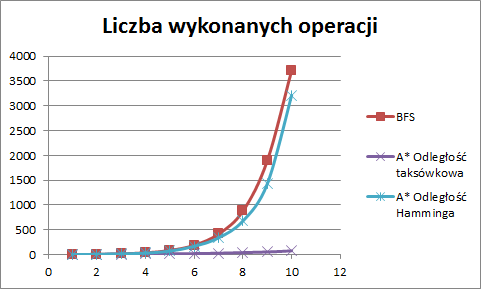
\includegraphics[scale=0.65]{pictures/operacje_BFS_vs_A.png}
	\caption{BFS vs A*}
	\label{fig:BFS vs A*}
\end{figure}

\begin{figure}[ht]
\centering
			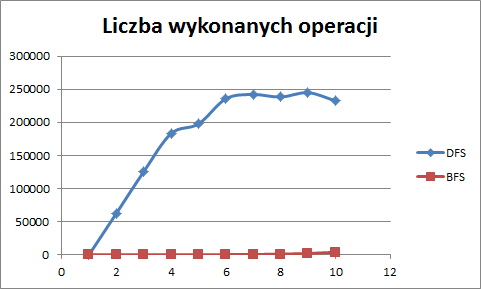
\includegraphics[scale=0.65]{pictures/operacje_BFS_vs_DFS.png}
	\caption{BFS vs DFS}
	\label{fig:BFS vs DFS}
\end{figure}

\begin{figure}[ht]
\centering
			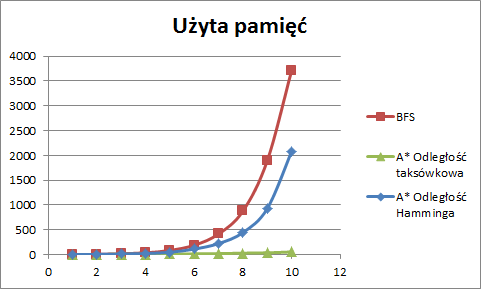
\includegraphics[scale=0.65]{pictures/space_BFS_vs_A.png}
	\caption{BFS vs A*}
	\label{fig:BFS vs A*}
\end{figure}

\begin{figure}[ht]
\centering
			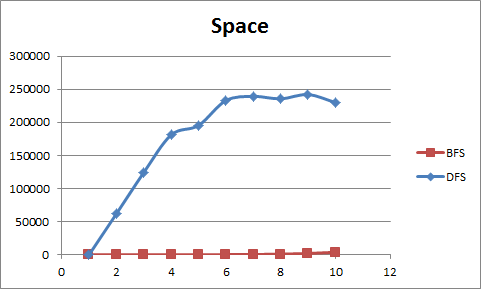
\includegraphics[scale=0.65]{pictures/space_BFS_vs_DFS.png}
	\caption{BFS vs DFS}
	\label{fig:BFS vs DFS}
\end{figure}

\cleardoublepage

\section{Wnioski}
  Najwydajniejszymi algorytmami okazały się, zgodnie z oczekiwaniami, algorytmy wykorzystujące heurystykę. Spowodowane jest to tym, że wybierane są tutaj drogi, które są najbliżej rozwiązania porzucając pozostałe. Funkcjonalności tej pozbawione są algorytmy nie wykorzystujące heurystyk, przez co rośnie czas poszukiwania. Najmniej wydajnym algorytmem okazał się DFS, ponieważ liczba rekurencji jest tutaj największa.


	
	
	
\begin{thebibliography}{0}
  \bibitem{l2short} T. Oetiker, H. Partl, I. Hyna, E. Schlegl.
    \textsl{Nie za krótkie wprowadzenie do systemu \LaTeX2e}, 2007, dostępny
    online.
  \bibitem{klesk_grafy} Przemysław Klęsk.
    \textsl{Algorytmy przeszukiwania grafów i drzew dla gier i łamigłówek}, \url{http://wikizmsi.zut.edu.pl/uploads/b/be/2_search.pdf}
   \bibitem{wiki_bfs} Wikipedia, wolna encykolpedia
    \textsl{Breadth-first search}, \url{http://en.wikipedia.org/wiki/Breadth-first_search}
    \bibitem{wiki_astar} Wikipedia, wolna encyklopedia
    \textsl{Algorytm A*}, \url{http://pl.wikipedia.org/wiki/Algorytm_A*}
\end{thebibliography}
\end{document}